%%%%%%%%%%%%%%%%%%%%%%%%%%%%%%%%%%%%%%%%%%%%%%%%%%%%%%%%%%%%%%%%%%%%%
%%                                                                 %%
%% Please do not use \input{...} to include other tex files.       %%
%% Submit your LaTeX manuscript as one .tex document.              %%
%%                                                                 %%
%% All additional figures and files should be attached             %%
%% separately and not embedded in the \TeX\ document itself.       %%
%%                                                                 %%
%%%%%%%%%%%%%%%%%%%%%%%%%%%%%%%%%%%%%%%%%%%%%%%%%%%%%%%%%%%%%%%%%%%%%
\RequirePackage{tikz}

\documentclass[pdflatex,referee,iicol,sn-basic]{sn-jnl}

%%%% Standard Packages
\usepackage{xcolor,hyperref}
\usepackage[autostyle=false, style=english]{csquotes}
%%%%

% Avoid having to ``quote'' verbosely (csquotes package)
\MakeOuterQuote{"}

% Make Orcid icon
\definecolor{lime}{HTML}{A6CE39}
\DeclareRobustCommand{\orcidicon}{%
	
\begin{tikzpicture}
	\draw[lime, fill=lime] (0,0) 
	circle [radius=0.16] 
	node[white] {{\fontfamily{qag}\selectfont \tiny ID}};
	\draw[white, fill=white] (-0.0625,0.095) 
	circle [radius=0.007];
	\end{tikzpicture}
	\hspace{-2mm}
}

\foreach \x in {A, ..., Z}{%
	\expandafter\xdef\csname orcid\x\endcsname{\noexpand\href{https://orcid.org/\csname orcidauthor\x\endcsname}{\noexpand\orcidicon}}
}

% Define the ORCID iD command for each author separately.
\newcommand{\orcidauthorA}{0000-0002-3420-4576}
\newcommand{\orcidauthorB}{0000-0001-9402-0851}

%%%%%=============================================================================%%%%
%%%%  Remarks: This template is provided to aid authors with the preparation
%%%%  of original research articles intended for submission to journals published 
%%%%  by Springer Nature. The guidance has been prepared in partnership with 
%%%%  production teams to conform to Springer Nature technical requirements. 
%%%%  Editorial and presentation requirements differ among journal portfolios and 
%%%%  research disciplines. You may find sections in this template are irrelevant 
%%%%  to your work and are empowered to omit any such section if allowed by the 
%%%%  journal you intend to submit to. The submission guidelines and policies 
%%%%  of the journal take precedence. A detailed User Manual is available in the 
%%%%  template package for technical guidance.
%%%%%=============================================================================%%%%

\jyear{2021}%

%% as per the requirement new theorem styles can be included as shown below
\theoremstyle{thmstyleone}%
\newtheorem{theorem}{Theorem}%  meant for continuous numbers
%%\newtheorem{theorem}{Theorem}[section]% meant for sectionwise numbers
%% optional argument [theorem] produces theorem numbering sequence instead of independent numbers for Proposition
\newtheorem{proposition}[theorem]{Proposition}% 
%%\newtheorem{proposition}{Proposition}% to get separate numbers for theorem and proposition etc.

\theoremstyle{thmstyletwo}%
\newtheorem{example}{Example}%
\newtheorem{remark}{Remark}%

\theoremstyle{thmstylethree}%
\newtheorem{definition}{Definition}%

\raggedbottom
%%\unnumbered% uncomment this for unnumbered level heads

\begin{document}

\title{Short-term neuronal and synaptic plasticity act in synergy for deviance detection in spiking networks}

%%=============================================================%%
%% Prefix	-> \pfx{Dr}
%% GivenName	-> \fnm{Joergen W.}
%% Particle	-> \spfx{van der} -> surname prefix
%% FamilyName	-> \sur{Ploeg}
%% Suffix	-> \sfx{IV}
%% NatureName	-> \tanm{Poet Laureate} -> Title after name
%% Degrees	-> \dgr{MSc, PhD}
%% \author*[1,2]{\pfx{Dr} \fnm{Joergen W.} \spfx{van der} \sur{Ploeg} \sfx{IV} \tanm{Poet Laureate} 
%%                 \dgr{MSc, PhD}}\email{iauthor@gmail.com}
%%=============================================================%%

\author[1]{\fnm{Felix Benjamin} \sur{Kern} \orcidA{}}\email{kernfel@gmail.com}

\author*[1]{\fnm{Zenas C.} \sur{Chao} \orcidB{}}\email{zenas.c.chao@gmail.com}

\affil[1]{\orgdiv{International Research Center for Neurointelligence (WPI-IRCN)}, \orgname{The University of Tokyo}, \orgaddress{\city{Tokyo}, \country{Japan}}}

%%==================================%%
%% sample for unstructured abstract %%
%%==================================%%

\abstract{TODO}


\keywords{keyword1, Keyword2, Keyword3, Keyword4}

\maketitle

\section{Introduction}\label{sec-intro}


\section{Methods}\label{sec-methods}

\subsection{Model}\label{sec-model}

We modeled neurons as leaky integrate-and-fire units whose membrane potential $V_m$ at time $t$ followed
\begin{equation}
    \tau_m \frac{dV_m}{dt} = (V_{rest}-V_m) + I_{syn}(t)
\end{equation}
with $tau_m = 30$~ms the membrane time constant and $V_{rest} = -60$~mV the resting membrane potential. Synaptic currents were modeled in a conductance-based manner, following
\begin{equation}
    I_{syn} = g_e(E_e-V_m) + g_i(E_i-V_m)
\end{equation}
with $E_e = 0$~mV and $E_i = -100$~mV the excitatory and inhibitory reversal potentials, respectively. Synaptic conductances evolved according to
\begin{align} 
    \tau_e \frac{dg_e}{dt} &= -g_e + \sum_{j \in \boldsymbol E} U x_j w \delta(t - \hat{t_j}) \nonumber \\
    \tau_i \frac{dg_i}{dt} &= -g_i + \sum_{j \in \boldsymbol I} w \delta(t - \hat{t_j}) \label{eqn-gsyn}
\end{align}
with $\tau_e = 2$~ms the excitatory time constant, echoing AMPA receptor dynamics \citep{Hausser1997-cn}, $\tau_i = 4$~ms the inhibitory time constant, echoing GABA-A receptor dynamics \citep{Destexhe1994-oc}, $\boldsymbol E$ and $\boldsymbol I$ the sets of presynaptic excitatory and inhibitory neurons, respectively, $w$ the synaptic weight, $\delta(\cdot)$ the Dirac delta function, and $\hat{t}$ the spike times.

Excitatory, but not inhibitory, synapses were subject to short-term depression (STD), simplified from \cite{Tsodyks1997-qt}; since synaptic transmission was not stochastic, we modeled the depression variable $x_j$ as a property of the presynaptic neuron $j$,
\begin{equation}
    \tau_x \frac{dx_j}{dt} = (1-x_j) - U x_j \delta(t - \hat{t}) \label{eqn-xsyn}
\end{equation}
with recovery time constant $\tau_x = 150$~ms and release fraction $U = 0.4$.

When a neuron's membrane potential reached the firing threshold $v_\theta$, a spike was emitted, and the potential was clamped to $V_m = V_{reset} = -74$~mV for a fixed refractory period of 3~ms (excitatory neurons). Inhibitory neurons were modeled as fast-spiking cells with a refractory period of 2~ms and a constant firing threshold $v_\theta = \theta_0 = -54$~mV \refp{Mensi2012-au}. In contrast, excitatory neurons were modeled with threshold adaptation (TA) as in \cite{Teeter2018-iz}, following
\begin{align}
    v_\theta &= \theta_0 + V_{TA}(t) \nonumber \\
    \tau_{\theta} \frac{dV_{TA}}{dt} &= -V_{TA} + \hat{\theta} \delta(t - \hat{t}) \label{eqn-TA}
\end{align}
with increment $\hat{\theta} = 1$~mV and decay time constant $\tau_{\theta} = 1$~s \refp{Pozzorini2015-ei}.

\begin{figure*}%
    \centering
    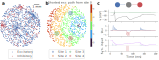
\includegraphics{fig1.pdf}
    \caption{}
    \label{fig1}
\end{figure*}
\textbf{Fig. 1}Model and paradigm. \textbf{a} Membrane and synaptic dynamics of a neuron innervated by an excitatory and an inhibitory neuron, illustrated above the plots, firing pre-determined spikes. The excitatory connection has weight $w = 3$ for demonstration purposes only; a single connection with $w = 1$ is normally unable to evoke postsynaptic firing. Top: Membrane voltage (black), firing threshold baseline (gray) and adaptive threshold (green) demonstrating TA. Middle: Excitatory ($g_e$, blue) and inhibitory ($g_i$, red) synaptic conductances, demonstrating excitatory STD. Bottom: Inputs to $g_e$ and $g_i$ (vertical bars in the appropriate colors), and the depression variable $x$ of the excitatory presynaptic neuron (dashed line). \textbf{b} Sample network layout, showing excitatory and inhibitory neurons and all outgoing synaptic connections from two neurons of each type. \textbf{c} Distance from stimulation site 0 in terms of minimum number of excitatory synapses. Stimulation is provided to the 10 neurons nearest to the center of each of 5 stimulation sites (round markers), which are regularly spaced on a circle with a radius of 2.5 mm.

Figure \ref{fig1}a shows the internal and presynaptic dynamics of an excitatory neuron in a contrived example for the purpose of illustration. The model was implemented in Brian2 \citep{Stimberg2019-tc}, accelerated with Brian2GeNN \citep{Stimberg2020-go}, and simulated with an integration time step of 1~ms. Synaptic delay was not modeled explicitly, but spikes were delivered, and voltages reset, in the time step following spike emission. We simulated neurons without any stochasticity in either their inputs or their parameters, other than network structure (described below), in order to ensure that our results were driven purely by the experimental paradigm, rather than any model-internal sources of noise.

800 excitatory and 200 inhibitory neurons were placed randomly in a two-dimensional circular space with a radius of 4~mm, and formed synapses of weight $w = 1$ with 50 randomly selected postsynaptic partners within a range of 2~mm (excitatory) or 1~mm (inhibitory), reflecting the notion that excitatory neurons project over longer distances, while inhibitory neurons mainly connect to their local neighborhood. Connectivity and weights remained fixed throughout. Stimulation sites were evenly distributed 2.5~mm from the center of the dish, and stimulation delivered a one-time increase in $g_e$ to the 10 closest neurons, sufficient to trigger 2-3 spikes each. See Figure \ref{fig1}b and c for a representative example of the resulting network structure. Networks were pseudo-randomly generated according to the above scheme and screened for minimal stimulus response: Networks where fewer than 500 neurons responded to stimulation at any of the five sites after full recovery were discarded. In total, 30 networks were used for the experiments described below.

\subsection{Paradigm}\label{sec-paradigm}

To investigate deviance detection, we used a classical oddball paradigm as illustrated in Figure \ref{fig1}d, presenting a total of 500 stimuli at regular intervals of 500~ms. Target stimuli (labeled "A" or "target" hereafter) and distractor stimuli (labeled B to E) were presented in three randomized sequences: The "standard" sequence (std), consisting of 400 presentations of A and 100 presentations of B; the "deviant" sequence (dev) with 100 A and 400 B, and the many-standards control sequence (msc) with 100 presentations of each of the stimuli A through E. In this way, A is presented as the predominant and therefore expected stimulus (std), as an infrequent violation of an expectation (of B, dev), and, to control for pure adaptation effects, as an equally infrequent stimulus with no strong expectation of any particular input (msc).

In each network, we simulated oddball sequences with two A/B stimulus pairs (sites 1 and 2 in one pair, and sites 3 and 5 in the other pair), where each stimulus site in a pair was used once as target (A) and once as non-target (B), and a single msc sequence involving all sites. Networks were reset to a fully recovered state between sequence presentations to guarantee their independence. This yielded 4 complete data sets per network, or a total of 120 data sets across all networks.

In order to disentangle the effects of STD and TA, we ran all simulations in four conditions: Without any short-term plasticity, with either TA only or STD only, and with both STD and TA (labeled STD+TA in the following, and corresponding to the full model as described above). To turn off STD, we replaced Equation \ref{eqn-xsyn} with a constant $x = 1$, but retained the scaling of inputs to $g_e$ with $U$ in Equation \ref{eqn-gsyn}. This corresponds to immediate recovery ($\tau_x = 0$) and was done to maintain the magnitude of the excitatory postsynaptic potential (EPSP) in the recovered state regardless of whether STD was turned on or off. To turn off TA, we replaced Equation \ref{eqn-TA} with a constant $V_{TA} = 0$, making the firing threshold completely unadaptive.

\section{Results}\label{sec-results}

\subsection{Deviance detection}\label{sec-dd}

\begin{figure*}%
    \centering
    \includegraphics{fig2.pdf}
    \caption{}
    \label{fig2}
\end{figure*}
\textbf{Fig. 2} Deviance detection in vitro and in silico. \textbf{a} Response of a 2 $\times$ 4~mm neuronal cell culture on a multi-electrode array, adapted from \cite{Kubota2021-dx}. Curves represent the average number of spikes per electrode in each 10~ms bin in response to target stimulation in the indicated sequence. Unlike in our study, oddball sequences here were split 10\%/90\%, and 10 equally frequent stimuli were used for the msc sequence. \textbf{b} Sample model response, showing average network-wide spike counts after stimulation with target (A) in the indicated sequence (same color code as panel \textbf{a}). Both in vitro and in the model, the dev response is very large, followed by an intermediate msc response and a low std response. \textbf{c} Mismatch, SSA and deviance detection indices (see Equation \ref{eqn-ddi}) across networks and stimuli (n = 120). In this and later boxplots, the median is indicated with an orange line, notches indicate the 95\% confidence interval for the median calculated by bootstrap with 10000 iterations, boxes indicate the inter-quartile range (IQR), whiskers extend to 1.5 times the IQR or to the data extrema, whichever is less, and fliers indicate individual data points beyond the whisker end points

We define deviance detection as a network's ability to pick out unexpected inputs from an otherwise homogeneous or otherwise unsurprising stream of inputs. Following related research \citep{Kubota2021-dx,Harms2014-ah,Jacobsen2001-sc}, we were careful to exclude effects due to stimulus identity (i.e., avoiding direct comparisons between different stimuli) or due to adaptation to frequent stimulus presentation (i.e., avoiding direct comparisons of A in the dev sequence to A in the std sequence). In other words, we used the msc sequence as a neutral baseline where the target stimulus was presented no more often than in the dev sequence, but no expectation of a competing stimulus B could be formed. To quantify deviance detection, we compared the mean number of spikes $R^A$ fired across the network in response to target stimulus A in the dev and msc sequences, defining a deviance detection index (DDI) as
\begin{equation}
    DDI = \frac{R^A_{dev} - R^A_{msc}}{R^A_{dev} + R^A_{msc}} \label{eqn-ddi}
\end{equation}
We define stimulus-specific adaptation (SSA, $R^A_{msc} - R^A_{std}$) and mismatch ($R^A_{dev} - R^A_{std}$) indices analogously, capturing respectively the effect of adaptation, and of both adaptation and deviance detection together.

Our first aim was to replicate deviance detection properties reported in dissociated neuronal cell culture by \cite{Kubota2021-dx}, reproduced in Figure \ref{fig2}a. In their case, cell cultures -- like our model, randomly connected networks with two-dimensional extent -- were stimulated at 10 different sites in msc sequences, and at two sites with 10\%/90\% probability in dev and std sequences. Deviance detection was assessed analogously to our definition of DDI and reached an average level of around 0.3 across two cultures.

In our model, we could readily identify networks and stimuli whose responses developed in a qualitatively similar fashion, with high activity in response to target in the dev sequence, low activity in the std sequence, and intermediate activity in the msc sequence, as illustrated with an example in Figure \ref{fig2}b. The model responses developed on a compressed time scale compared to neuronal culture, which we tentatively attribute to unfaithful aspects of the model, including a lack of conduction delay or spontaneous activity, a much smaller number of participating neurons, and structural differences.

Across networks and stimuli (Figure \ref{fig2}c), we found that our model reliably produced mismatch responses (t = 11.3, p = 6.7e-21; one-sided t-test for mismatch index > 0, n = 120) while both SSA index (t = 7.84, p = 1.05e-12) and DDI (t = 6.49, p = 1.05e-09) were also positive. The average DDI value reached around 0.1, which was less than the values reported by \cite{Kubota2021-dx}, but note that our target stimuli were presented more frequently (20\%) than theirs (10\%) in the dev and msc sequences.

\begin{figure*}%
    \centering
    \includegraphics{fig3.pdf}
    \caption{}
    \label{fig3}
\end{figure*}
\textbf{Fig. 3} Deviance detection under model ablation. \textbf{a} Sample network responses to target stimulation, with the deviance detection index in each instance noted in the plot titles. The color code is the same as in Figure \ref{fig2}. \textbf{b} SSA indices across all networks and stimuli. Asterisks indicate data greater than 0 at a significance level of p<0.05, see main text for detailed statistics. \textbf{c} Deviance detection indices across all networks and stimuli.

Having confirmed the presence of deviance detection in our model, we then turned to an ablation approach to try to identify how the two short-term plasticity mechanisms in the model, STD and TA, enabled the networks to learn relevant regularities. In the remainder of the paper, we will proceed to detail the processes leading to deviance detection on a sample network, then confirm the highlighted trends statistically with reference to the full set of 120 networks and stimuli. The sample network was chosen to be roughly representative of the population as follows: We assessed each network's average response to stimulation with A and B in the msc sequence and calculated z-scores with respect to the population. We then focused on networks whose absolute z-score was less than 1 for both A and B responses, and hand-picked a sample that exhibited both an increased DDI in STD+TA over TA only, and positive SSA indices in both STD+TA and TA only conditions.

Figure \ref{fig3}a shows the responses to target stimulation of the sample network under ablation. With no plasticity, the responses are indistinguishable between sequences, yielding a DDI of 0, and indicating that stimulation did not have any long-lasting effects in membrane voltage or synaptic conductance. With STD only, the response in the dev sequence developed earlier and very slightly larger, yielding a DDI of 0.03. With TA only, the response became noticeably smaller, but the sequences became readily distinguishable, with high dev, intermediate msc, and low std responses, yielding a DDI of 0.19. Finally, in the full model, the dev response stood out more clearly, leaving much smaller msc and std responses and yielding a DDI of 0.4.

The SSA index (Figure \ref{fig3}b) was exactly 0 as expected in the ablation with no plasticity, and positive with any plasticity applied (STD only: t = 3.17, p = 0.000983, median 0.0039; TA only: t = 6.74, p = 3e-10, median 0.097; STD+TA: t = 7.84, p = 1.05e-12, median 0.135; one-sided t-tests, n = 120). Since the SSA index measures the degree of adaptation to frequent stimulus presentation, this indicates that both plasticity mechanisms were capable of imbuing the networks with some level of history dependence.

Finally, across networks and stimuli, the DDI (Figure \ref{fig3}c) was exactly 0 with no plasticity, not significantly different from 0 with STD only (t = -1.89, p = 0.0609, median -2.1e-04; two-sided t-test, n = 120), but clearly positive for TA only (t = 5.52, p = 1.01e-07, median 0.077; one-sided t-test, n = 120) and the full model (t = 6.49, p = 1.05e-09, median 0.114). To our surprise, the DDI of the full model was significantly greater than that of either plasticity mechanism alone (STD: t = 6.7, p = 4.53e-10; TA: t = 3.2, p = 0.00103), and greater too than the sum of the DDI values across both STD only and TA only models (t = 3.6, p = 0.000199). This suggests that TA and STD act not as independent mechanisms in this paradigm, but rather interact constructively to enhance the network's ability to encode input regularities.

In the following, we will use a sample network and target stimulus to first build an understanding of how TA leads to deviance detection when acting alone, i.e. in the ablated TA only model. Then, we will build on this understanding to elucidate how the addition of STD, which was shown above to be ineffective for deviance detection on its own, can lead to an increased deviant response in the full model.

\subsection{The role of TA in deviance detection}\label{sec-ta}

To understand why the same stimulus A evoked a higher response in dev than in msc with TA only, we first compared the average responses in the two conditions, sorting neurons by their response onset to permit a high-resolution view of the population activity. As shown in Figure \ref{fig4}a (left and middle), we found that the response developed in a qualitatively similar fashion in both conditions. The contrast (right) revealed a tendency of dev spikes to occur earlier, particularly shortly after stimulation, as shown by the succession of orange (higher dev activity) by blue (higher msc activity) in the lower parts of the panel. In later parts of the response (top half of the panel), the dev response was larger, but not obviously shifted in time. Since the stimulus was identical in both conditions, and TA was the only plsaticity mechanism in play, these differences had to be due to (1) different firing thresholds, and/or (2) different synaptic currents as a consequence of different prior activity within the trial.

We quantified the former with the strength of adaptation $V_{TA}$ (Equation \ref{eqn-TA}), i.e., the amount by which the firing threshold was raised due to TA. As shown in Figure \ref{fig4}b, there was a clear and widespread lowering of thresholds at the start of target dev trials relative to msc, visible both in the raw data (left and middle panels) and in the contrast (right panel, early blue portions). In contrast, once the bulk of activity had occurred, many neurons showed higher thresholds in dev (right panel, later orange portions), since they spiked more often. Finally, note that inhibitory neurons, which were modeled without TA, naturally showed no difference in $V_{TA}$.

To assess the difference in synaptic currents in a way that allowed direct comparison to $V_{TA}$, we referred to the membrane voltage $V_m$, which is largely independent from and complementary to the firing threshold, and driven mostly by presynaptic inputs (resets after spikes notwithstanding). As the direct cause of neuronal spiking, the overall pattern of $V_m$ (Figure \ref{fig4}c) largely reflected that seen in spiking activity. The contrast (right panel) shows not only a notable relative increase in membrane voltages in dev around the typical response time (note the orange band running along the response front), but also an increased hyperpolarization starting immediately after due to post-spike resets.

\begin{figure*}%
    \centering
    \includegraphics{fig4.pdf}
    \caption{}
    \label{fig4}
\end{figure*}
\textbf{Fig. 4} Responses and threshold adaptation with TA only.
\textbf{a} Target trial average post-stimulus spike histogram in the sample network, showing trial time along the horizontal axis, and neurons along the vertical, sorted by the time of the first recorded spike across all trials and conditions. Left and middle column, target trials in dev sequence and msc sequence, respectively; right column, contrast between these two.
\textbf{b} Target trial average of the threshold adaptation voltage $V_{TA}$, with axes, neuron order and columns as in panel a.
\textbf{c} Target trial average of the membrane potential $V_m$, with axes, neuron order and columns as in panel a. The first 10 ms of the neurons under direct stimulation are masked out to avoid saturation of the color mask.
\textbf{d} Relationship across excitatory neurons of the sample network between the contrast (dev - msc) in $V_{TA}$ at the start of target trials and the contrast in average number of spikes fired in target trials, and associated linear regression.
\textbf{e} Network-wide mean contrast (dev - msc) in $V_{TA}$ across networks and stimuli, plotted against the Pearson correlation coefficients $\rho$ of the relationship shown in the previous panel ($\Delta V_{TA}$ vs response size contrast across excitatory neurons). Each marker corresponds to one network and target stimulus. Red markers indicate a significant correlation (p < 0.05). Inset histograms show the distribution of the corresponding values, with orange portions indicating the 95\% confidence interval of the median, calculated by bootstrap with 10000 iterations.
\textbf{f} In the sample network, contribution of the contrast in $V_{TA}$ and $V_m$ to bins with increased firing in dev (i.e., positive/red bins in the spike probability contrast, panel a), weighted by that same contrast.
\textbf{g} Contribution of $V_{TA}$ relative to the sum of the absolute values of the weighted contributions in panel f.
\textbf{h} Relative contribution of $V_{TA}$ across networks and stimuli, showing median (solid line) and inter-quartile range (shaded area)

Based on these measures, we then asked why there were more spikes in dev trials. We first focused on the contribution of $V_{TA}$ alone in an effort to confirm that thresholds are lower in dev, and that this reduction in thresholds causes increased firing. We correlated the level of $V_{TA}$ at the start of target trials (i.e., at the left edge of the histograms in Figure \ref{fig4}b) with the average target trial response of each excitatory neuron in terms of spikes fired. In the sample network (Figure \ref{fig4}d), we found that thresholds were clearly lower in dev than msc (t = -17.3, p = 2.57e-57, median -0.166 mV; one-sided t-test, n = 800), and this decrease was accompanied by an increase in the target trial response at the level of individual neurons (Pearson's $\rho$ = -0.424, p = 3.1e-36). As shown in Figure \ref{fig4}e, this relationship held across networks and stimuli: Average $V_{TA}$ was lower in dev than msc (t = -7.32, p = 1.58e-11, median = -0.074 mV; one-sided t-test, n = 120), and the neuron-level correlation between the contrasts in $V_{TA}$ and target response was almost universally negative (t = -23.1, p = 3.72e-46, median = -0.357). This indicates that networks were less adapted during oddball sequences, and that this lack of adaptation played an important role in the increased response to deviant inputs.

Yet, as we saw in Figure \ref{fig4}c, the membrane voltages also differed between the two conditions. In order to assess the relative contribution of $V_{TA}$ to the increased dev response, we chose to focus exclusively on time points with higher firing probability in the dev sequence, discarding data points with equal or lower firing probability relative to the msc sequence. We then weighted the remaining contrasts in $V_{TA}$ and $V_m$ by the magnitude of the response difference, and summed across neurons. The resulting time courses, shown in Figure \ref{fig4}f, show how much these two measures contributed to the increased dev response. While thresholds were slighly lowered throughout the response, the membrane potential was dramatically increased. In relative terms (Figure \ref{fig4}g), $V_{TA}$ constituted a major driver of increased firing only right at the onset of the response, with later contributions amounting to less than 20\% of the total voltage difference. This pattern was consistent across networks and stimuli, as shown in Figure \ref{fig4}h. This indicates that adaptation initiated and dominated the increase in firing in the beginning, whereas the late response was enlarged primarily as a result of increased presynaptic excitation.

Having established that the increased response to A in dev trials was driven by lower thresholds, we next turned to the cause of this reduction. A priori, since threshold adaptation is a direct reflection of activity, and since the response to target trials was larger in dev than in msc, the lower thresholds in dev must have been caused by lower activity in non-target trials, i.e. lower responses to B in dev than to B through E in msc. Yet, with activity modulated by thresholds as shown above, we might expect to observe higher dev responses regardless of stimulus. To resolve this apparent paradox, we will turn to an analysis of the spatial arrangement of activity and adaptation.

First, we mapped the average value of $V_{TA}$ at the start of target trials to the spatial location of the neurons, as shown in Figure \ref{fig5}a. In the msc sequence, $V_{TA}$ was roughly evenly distributed across the network, consistent with the random, distributed nature of stimulation. Conversely, in the dev sequence, neurons near the non-target stimulation site (B) were strongly adapted, whereas the majority of the network was less adapted, consistent with the data shown above.
Next, we turned to the likely cause of this difference, the non-target responses (Figure \ref{fig5}b), mapped into space as the average number of spikes fired in each neuron. As expected, the pattern of activity in non-target trials, constituting 80\% of all trials, closely matched that of the thresholds. Notably, although the comparison is between 400 B trials in dev, and only 100 B trials (alongside 300 C, D and E trials) in msc, only a small handful of neurons responded more to non-target stimulation in dev, most of these very close to the stimulation site of B.

Correlating the non-target response and thresholds excitatory neurons (Figure \ref{fig5}c), we found that the reduced non-target response magnitude in dev (t = -7.61, p = 3.5e-12, median = -0.044; one-sided t-test, n = 800) almost perfectly predicted the resulting reduction in threshold adaptation levels (Pearson's $\rho$ = 0.99, p = 0).
This finding held across networks and stimuli, as shown in Figure \ref{fig5}d, with a median correlation coefficient of 0.994 and a consistent reduction in the average non-target response between msc and dev sequences (t = -11.6, p = 1.46e-21, median = -0.058; one-sided t-test, n = 120), clearly validating our notion that the non-target trial response is the primary driver of threshold adaptation.

\begin{figure*}%
    \centering
    \includegraphics{fig5.pdf}
    \caption{}
    \label{fig5}
\end{figure*}
\textbf{Fig. 5} Non-target response magnitude determines thresholds.
\textbf{a} $V_{TA}$ at the start of A trials (mean over trials) in the sample network, with each neuron shown in its spatial location. Left and middle column, raw averages for dev and msc sequences, respectively; right column, contrast between dev and msc averages. A and B stimulus locations for this and following figures are highlighted in the left plot; see Figure \ref{fig1} for the locations of the remaining stimuli used in the msc sequence.
\textbf{b} Average response (in spikes per trial) to non-target trials (B in dev, B, C, D, and E in msc). Columns are arranged as in panel a.
\textbf{c} Relationship across excitatory neurons of the sample network between the contrast (dev - msc) in average number of spikes fired in response to non-target stimulation and the contrast in $V_{TA}$ at the start of target trials, and associated linear regression.
\textbf{d} Network-wide mean contrast (dev - msc) in the non-target response magnitude across networks and stimuli, plotted against the Pearson correlation coefficients $\rho$ of the relationship shown in the previous panel (non-target response size contrast vs $\Delta V_{TA}$ across excitatory neurons). Each marker corresponds to one network and target stimulus. Red markers indicate a significant correlation (p < 0.05). Inset histograms show the distribution of the corresponding values, with orange portions indicating the 95\% confidence interval of the median, calculated by bootstrap with 10000 iterations

\begin{figure*}%
    \centering
    \includegraphics{fig6.pdf}
    \caption{}
    \label{fig6}
\end{figure*}
\textbf{Fig. 6} Stimulus replacement and adaptation both lead to a reduced dev non-target response.
\textbf{a} Non-target response contrasts in the sample network: The replacement contrast (top right) compares the response to B in msc (top left) to all non-target responses in msc (top center). The adaptation contrast (bottom right) compares the response to B in dev (bottom left) to the response to B in msc (bottom center). Both contrasts together add up to the non-target contrast (dev - msc) shown in Figure \ref{fig5}b. Note that the contrast column (right) shares a color scale to allow a direct comparison.
\textbf{b} Network-wide mean replacement (left) and adaptation (right) contrasts across networks and stimuli, as well as the mean replacement contrast filtered for neurons near B, i.e., neurons within one excitatory synapse of the neurons under direct stimulation of B (center).
\textbf{c} Mean $V_{TA}$ contrast (dev - msc) at the start of A trials, filtered for neurons near B. Each marker corresponds to one network; the sample network is highlighted in red. The histogram in the background shows the distribution of the data, with the orange portion indicating the 95\% confidence interval of the median, calculated by bootstrap with 10000 iterations

Finally, we examined the cause of the reduced response in non-target trials. Going from the msc sequence to the dev sequence, two things change: Firstly, stimulations with non-target C, D and E are replaced with B, which would cause different responses even in the absence of adaptation. Secondly, the more frequent presentation of B changes adaptation, likely reducing the average response to B.
In order to separate these two, we split the non-target contrast shown in Figure \ref{fig5}b into two components: a replacement effect, contrasting the response to B in the msc sequence with the response to all non-target stimuli in the same sequence; and an adaptation effect, contrasting the response to B in dev with the response to B in msc. For the sample network, these contrasts are shown in Figure \ref{fig6}a. Unsurprisingly, replacement yielded a decreased response near the stimulation sites for C, D and E, and an increased response in areas near the stimulation site for B. By contrast, adaptation caused a decreased response in virtually the entire network, particularly in the vicinity of the stimulation site for B.

Across networks and stimuli (Figure \ref{fig6}b), we saw a wide range of replacement effects, including both increased and decreased firing, likely as a result of differing sensitivities of the networks to the various non-target stimuli. On average, stimulus replacement did not have a significant effect (t = -0.255, p = 0.799; two-sided t-test). In contrast, adaptation yielded a reduced response on average (t = -9.01, p = 2.02e-15; one-sided t-test), indicating that the more frequent presentation of B indeed lowered the network's response to this stimulus.

Finally, given the clear spatial pattern exhibited by the replacement effect in the sample network, we surmised that adaptation is driven mainly by neurons close to the stimulation site B responding more frequently due to the more frequent presentation of the stimulus. To show this, we first identified all neurons located within a single excitatory synapse of the stimulated neurons (cf. Figure \ref{1}c), and calculated the average replacement effect for these alone. In this subpopulation, replacement yielded a clear response increase, shown in the central box of Figure \ref{fig6}b (t = 8.21, p = 1.5e-13; one-sided t-test). As shown in Figure \ref{fig6}c, this response increase directly translated into elevated thresholds in dev trials compared to msc (t = 5.01, p = 9.59e-07).

Earlier, we showed that the early response is strongly influenced by TA (Figure \ref{fig4}h). Here, we showed that $V_{TA}$ near the stimulation site was increased in dev as a result of the more frequent presentation of B. We posit that this increase in TA affects the early response, reducing the response further downstream and freeing up the rest of the network to respond more strongly to the infrequent target stimulus.

To conclude, TA plays two complementary roles in deviance detection, affecting the standard and deviant response separately: In its first role, as we have shown with the adaptation contrast above, TA reduces the response to frequently presented stimuli regardless of context, leading to a stronger response to infrequently presented stimuli (SSA). Since this happens without the need for large-scale adaptation -- only a small fraction of the network near the stimulation site adapts strongly to frequently presented inputs -- the network as a whole is allowed to relax in the oddball condition. In its second role, TA causes network-wide adaptation in the control condition, where many different stimuli are presented, all of which are infrequently presented and therefore able to evoke large responses. Deviant detection then arises as a relief from this blanket suppression, or as a result of adaptation shifting from the entire network to a small region around the frequently presented standard.

\subsection{The role of STD in deviance detection}\label{sec-std}

As noted previously, short-term depression alone exerted no deviance detection effect, but its addition did enhance the deviance detection effect established by TA. To understand the basis of this apparent synergy, we contrasted the TA only condition examined in the previous section against the same networks with both TA and STD. On average, adding STD caused a reduction in response magnitude across the board, as we would expect from a depression mechanism (data not shown). However, this reduction was not uniform: Target responses were reduced most in the std sequence, and least in the dev sequence.

To understand the reason for this asymmetry, we first focused on the target response and asked how and why the target response contrast (dev - msc) changed as STD was added to the model. As shown in Figure \ref{fig7}a, the target response was greater in dev than msc in both the full and the ablated model (indicating a positive DDI in both models, cf. also Figure \ref{fig3}). In most neurons, the contrast was greater in the full model, such that the difference (full - ablated) was positive, as indicated by the largely orange plot in the right column.
Following the logic established in the previous section, we may expect a greater target response in dev to be caused by lower $V_{TA}$ relative to msc. Indeed, comparing the contrast (dev - msc) in $V_{TA}$ before target trials across models (Figure \ref{fig7}b), we see that, while the contrast is negative (i.e., lower in dev) in both models, the magnitude of the contrast is greater in the full model. For clarity, the difference is therefore negative, as indicated by the largely blue plot in the right column.
Lastly, we trace this one step further back in Figure \ref{fig7}c: Again as established in the previous section, a greater contrast in $V_{TA}$ may be explained by a similarly enhanced contrast (dev - msc) in the non-target response. We found exactly this: The non-target response was smaller in dev than msc by a greater margin in the full model, as indicated by the largely blue plot in the right column.

This pattern was reflected also in the aggregate across networks and stimuli. Firstly, the contrast (dev - msc) in the target response (Figure \ref{fig7}d, left) was positive in both models, but the full model contrast was greater than the ablated model contrast (t = 2.99, p = 0.00168; one-sided t-test, n = 120). Referring to the previous section, we identify the cause for this in an enhanced contrast in $V_{TA}$, as shown in Figure \ref{fig7}e; the contrast (dev - msc) in the full model was more negative than that in the ablated model (t = -3.49, p = 0.000342). Lastly, returning to Figure \ref{fig7}d (right), we see that the driver of $V_{TA}$, namely the non-target response size, also showed an enhanced contrast (dev - msc) in the full model relative to the ablation (t = -3.19, p = 0.000921). To sum up, the reason for the larger target dev response, relative to msc, was the smaller non-target dev response, relative to msc; furthermore, since the relationships established in the previous section remained largely unchanged, this effect appeared to be mediated primarily through TA.

\begin{figure*}%
    \centering
    \includegraphics{fig7.pdf}
    \caption{}
    \label{fig7}
\end{figure*}
\textbf{Fig. 7} Adding STD to the model enhances the effect of TA.
\textbf{a} Contrast (dev - msc) of the response to A, in terms of mean number of spikes per trial, in the sample network, with each neuron shown in its spatial location. Left and middle column, full model with STD and TA, and ablated model with only TA, respectively. Right column, subtraction of these two. Stimulus locations are as shown in Figure \ref{fig5}a.
\textbf{b} Contrast of mean $V_{TA}$ at the start of target trials, in columns as in panel a.
\textbf{c} Contrast of the response to non-target stimuli, in columns as in panel a.
\textbf{d} Network-wide mean contrast of the response to target (left) and non-target stimuli (right) across networks and stimuli, arranged equivalently to the columns in panels a-c. Blue and green boxes represent the full and ablated model, respectively, and white boxes the difference between these two.
\textbf{e} Network-wide mean contrast of $V_{TA}$ before A trials across networks and stimuli, arranged as in panel d

This naturally raises the question of why, with the addition of STD, the non-target dev response was reduced more than other responses. We hypothesized that, due to its relatively short time constant, the direct effect of STD across trials was limited to repeated trials of the same stimulus, such as the frequent stimulus in oddball sequences.

We had good reasons for this assumption: Firstly, notice that the ablated model with STD only produced only a positive SSA index (i.e., the target response in msc was greater than in std), but not a significantly positive DDI (i.e., no difference between target dev and msc responses). Secondly, we note that updates to the spike-triggered depression variable $x_j$ (cf. Equation \ref{eqn-xsyn}) would decay to a negligible $e^\frac{-1 s}{\tau_x} = 0.0013$ times the original value within two trials, making it unlikely that inputs separated by intervening trials could be "remembered" in the network. Conversely, the frequently presented stimulus B could lead to a build-up of depression strong enough to suppress its own response. Referring back to Figure \ref{fig3}b, we see that there was indeed a significant, if small, effect of presentation frequency even in the ablated model with STD only, yielding a positive SSA index on average.
% To show this in the sample network, we correlated the number of spikes in dev target trials with the spike-triggered depression variable $x_j$ at the start of later trials (cf. Equation \ref{eqn-xsyn}) across excitatory neurons. We found that, while the correlation was very clear in the trial immediately following target (Pearson's $\rho$ = -0.984, p = 0; n = 800), it was almost completely lost by the next trial ($\rho$ = -0.0525, p = 0.138) under the influence of both decay and unrelated activity in the intervening trial.

To show that STD being carried over between trials was responsible for the reduction of non-target dev pulses relative to msc, we needed to estimate the extent to which activity of a given neuron (or, alternatively, its membrane potential $V_m$) was affected by changes in STD. Unlike $V_{TA}$, which directly affected the neuron to which the value belongs, $x_j$ exerted its effects on the other side of a synapse. Therefore, we devised a measure $D$ to estimate the postsynaptic impact of STD in terms of membrane potential lost, mirroring the effect of $V_{TA}$ in the sense that decreasing $V_m$ and increasing the firing threshold both increase the depolarization necessary to bring a neuron to fire.
A depression measure is necessarily activity-dependent -- a postsynaptic neuron's membrane potential is driven only by presynaptic partners that fire -- so it must be calculated based on observed activity. Here, we used the average trial response $R_j^S$ of neuron $j$ to a given stimulus $S$, in number of spikes, as the presynaptic drive. Before depression, a single excitatory presynaptic spike evokes a postsynaptic potential (EPSP) peaking at approximately $k = 1.4$ mV at rest (recall that $w = 1$ for all synapses), and STD linearly scales this EPSP by presynaptic $x_j$. Thus, we estimated the average peak EPSP evoked by a spike in presynaptic neuron $j$ as $R_j^S k x_j^S$. For this estimate, we ignored added depression due to repeated spikes within a trial, instead defining $x_j^S$ as the average depression at the start of trials. Finally, summing over presynaptic neurons, we estimated the peak EPSP lost to depression in a given neuron $i$ as
\begin{equation}
    D_i^S = \sum_{j \in pre} R_j^S k (1-x_j^S)
\end{equation}
Notice that $D$ is measured in volts due to scaling with $k$, and is therefore roughly comparable to $V_{TA}$, albeit more approximate. Lastly, since we contrasted this measure between conditions (see below), we aimed to avoid effects purely due to differences in presynaptic activity. Therefore, we calculated $R^S$ as the average response across relevant trials in all conditions, leaving the contrast entirely in the hands of $x^S$.

\begin{figure*}%
    \centering
    \includegraphics{fig8.pdf}
    \caption{}
    \label{fig8}
\end{figure*}
\textbf{Fig. 8} Estimated STD-mediated depression $D$ has small direct effects.
\textbf{a} Average depression $D$ in target (A) trials (top row) and B trials (bottom row) in the dev (left) and msc sequence (center), and their contrast (right). The color scale is shared across columns (and between dev and msc) for direct comparability.
\textbf{b} Statistics across networks and stimuli of the contrast (dev - msc) in $D$ in A trials (left) and B trials (right)

As noted above, we hypothesized that, in the full model, STD is directly responsible only for a reduction of non-target dev trials, relative to msc, whereas differences between target dev and msc trials are not a result of STD directly. To show this, we calculated $D$ for A and B trials, and contrasted it across dev and msc conditions as with $V_{TA}$ before.
In Figure \ref{fig8}a, we see that target trials (top) experienced depression across large parts of the sample network in both conditions. The msc sequence, however, clearly evoked greater depression, as borne out in the contrast (dev - msc), which was negative throughout. Conversely, depression in B trials (bottom) were spatially more clustered around the stimulation site in both conditions. In the msc sequence, we can attribute the difference between A and B primarily to the response size: The context was the same, but responses to B tended not to spread out as much in this network. However, in the dev sequence, the B response was limited almost exclusively to a very local patch around the stimulation site (see also Figure \ref{fig6}a), with depression by definition similarly limited. As a result, the contrast (dev - msc) showed slightly reduced $D$ in the periphery, but strikingly elevated $D$ near the stimulation site, indicative of greatly increased synaptic depression in dev.

In order to show that this was a robust effect, we turn to statistics across networks and stimuli. We calculated the trial-average depression values $D^A$ and $D^B$ in dev and msc conditions, subtracted them, then calculated the mean over neurons, excluding neurons with less than 0.2 spikes per trial in both conditions [because $\Delta D^B$ $\approx$ zero if I don't do this. Not sure how to justify...]. The resulting contrasts are summarized in the left half of Figure \ref{fig8}b. We note first that, using the same exclusion criteria, we found that neurons received more depression in B trials than in A trials in the dev sequence (t = -4.4, p = 1.17e-05; one-sided t-test, n = 120), but not in the msc sequence (t = -1.14, p = 0.129). Furthermore, $D^B$ was greater in dev than msc (t = 2.94, p = 0.002). Both findings confirm that STD carried over between the frequent standard trials, but not, or less so, between control trials.

However, we also found that $D^A$ was greater in msc than dev (t = -3.4, p = 0.000458), suggesting that STD did exert stimulus-independent suppression in the msc sequence, similar to what we described earlier for TA. The magnitude of the effect, however, was very different. In the right half of Figure \ref{fig8}b, we show the contrast of $V_{TA}$ before A trials, which was clearly much greater than the contrast in $D^A$. We wondered, however, how much $V_{TA}$ was affected by the addition of STD. To assess this, we subtracted the contrast (dev - msc) of $V_{TA}$ in the full model from the same contrast calculated in the ablated model with TA only. This additional decrease in $V_{TA}$ from msc to dev was substantially greater than the corresponding decrease in $D^A$ (t = -1.93, p = 0.0277), indicating that the direct effect of STD on the target dev response was less than indirect effects.

To sum up, adding STD to the model had a number of direct and indirect effects. Firstly, it reduced responses in all conditions, likely by reducing the synaptic output of neurons at stimulus sites, which reliably fired several spikes immediately following stimulation. Secondly, it directly reduced the response to frequently presented dev B trials through stimulus-specific adaptation. Thirdly, STD was very slightly reduced in A trials in dev over msc, mirroring the direct stimulus-independent adaptation effect detailed in the previous section for TA. And finally, the decreased dev B trial response allowed TA in the wider network to recover more, which in turn led to increased responses in dev A trials. This indirect effect was substantially greater than the direct effect on target trials, as shown above, indicating that it was solely or largely responsible for the increased DDI.

\section{Discussion}\label{sec-discussion}






\backmatter

\bmhead{Supplementary information}
TODO

\bmhead{Author contributions}
All authors contributed to the study conception and design. Material preparation, data collection and analysis were performed by Felix Benjamin Kern. The first draft of the manuscript was written by Felix Benjamin Kern and all authors commented on previous versions of the manuscript. All authors read and approved the final manuscript.

\bmhead{Code availability}
TODO

\section*{Declarations}

\bmhead{Funding}
This study was funded by a World Premier International Research Center Initiative research startup grant.

\bmhead{Competing interests}
The authors have no relevant financial or non-financial interests to disclose.

\bmhead{Ethics approval}
Not applicable.

\bmhead{Consent to participate}
Not applicable.

\bmhead{Consent for publication}
Not applicable.

% \begin{appendices}

% \section{Section title of first appendix}\label{secA1}


% %%=============================================%%
% %% For submissions to Nature Portfolio Journals %%
% %% please use the heading ``Extended Data''.   %%
% %%=============================================%%

% %%=============================================================%%
% %% Sample for another appendix section			       %%
% %%=============================================================%%

% %% \section{Example of another appendix section}\label{secA2}%
% %% Appendices may be used for helpful, supporting or essential material that would otherwise 
% %% clutter, break up or be distracting to the text. Appendices can consist of sections, figures, 
% %% tables and equations etc.

% \end{appendices}

%%===========================================================================================%%
%% If you are submitting to one of the Nature Portfolio journals, using the eJP submission   %%
%% system, please include the references within the manuscript file itself. You may do this  %%
%% by copying the reference list from your .bbl file, paste it into the main manuscript .tex %%
%% file, and delete the associated \verb+\bibliography+ commands.                            %%
%%===========================================================================================%%

\bibliography{refs}% common bib file
%% if required, the content of .bbl file can be included here once bbl is generated
%%\input sn-article.bbl

%% Default %%
%%\input sn-sample-bib.tex%

\end{document}
